% \documentclass{beamer}
% \usetheme{Szeged}

% \usepackage{media9}
% \usepackage{graphicx}

% \begin{document}

%-------------------------------------------------------------------------------
%							THIRD SECTION
%-------------------------------------------------------------------------------
\section{Le problème en 1D}

\subsection{Simulation}

\begin{frame}[fragile]
    \frametitle{Exemple de simulation 1D}
  \begin{center}
    \includemedia[
      width=0.95\linewidth,
      activate=pageopen,
      addresource=Video1D.mp4,
      flashvars={
         source=Video1D.mp4
        &autoPlay=true
      },
      passcontext, % enable VPlayer's right-click menue
    ]{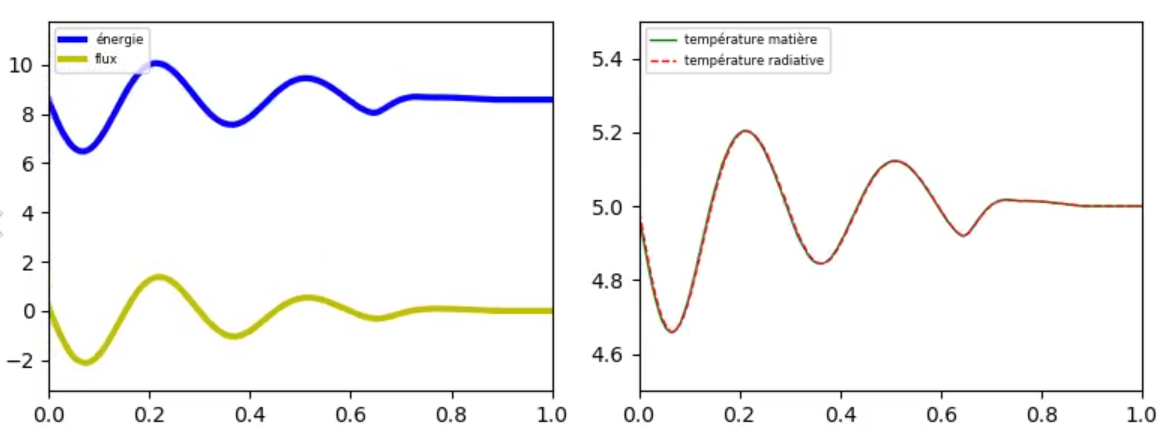
\includegraphics{Thumbnail1D.png}}{VPlayer.swf}%
  \end{center}
\end{frame}

\begin{frame}[fragile]
    \frametitle{Entree sortie 1D}

    \begin{columns}
    \begin{column}{0.7\textwidth}
        \begin{figure}
        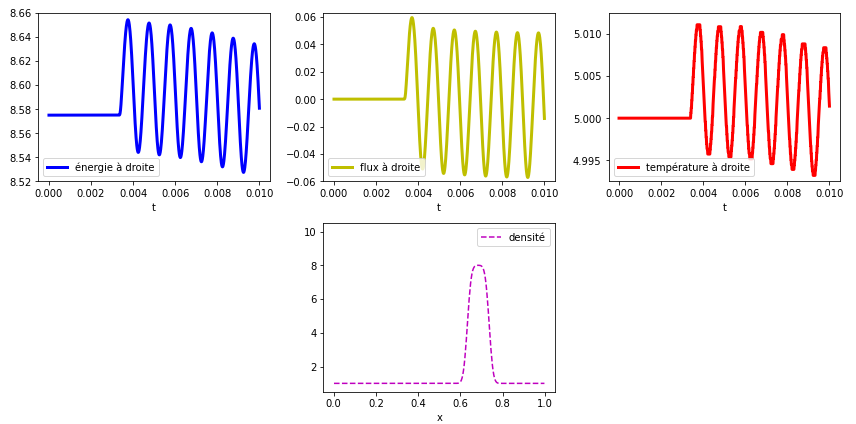
\includegraphics[width=8cm]{EntreeSortie1D}       
        \caption{Entrees/sortie pour le reseau de neurones}
        \end{figure}
     \end{column}
     \begin{column}{0.3\textwidth}
        \begin{figure}
        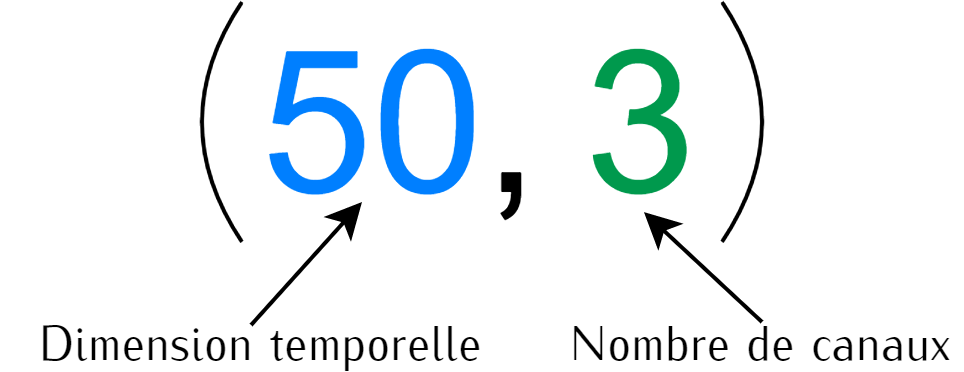
\includegraphics[width=3cm]{Entrees1D}       
        \caption{Taille d'une entree}
        \end{figure}
     \end{column}
    \end{columns}

\end{frame}

\subsection{Apprentissage}

\begin{frame}[fragile]
    \frametitle{Meilleures/pires predictions du reseau de neurones}

    \begin{columns}
    \begin{column}{0.5\textwidth}
        \begin{figure}
        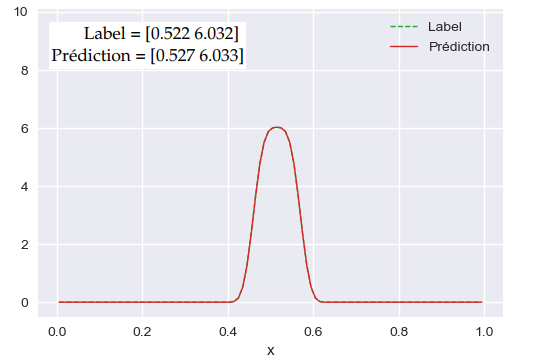
\includegraphics[width=4cm]{Meilleur1D2}       
        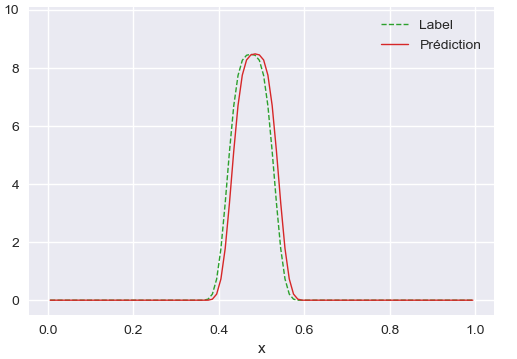
\includegraphics[width=4cm]{Meilleur1D1}       
        \caption{Les meilleures predictions}
        \end{figure}
     \end{column}
     \begin{column}{0.5\textwidth}
        \begin{figure}
        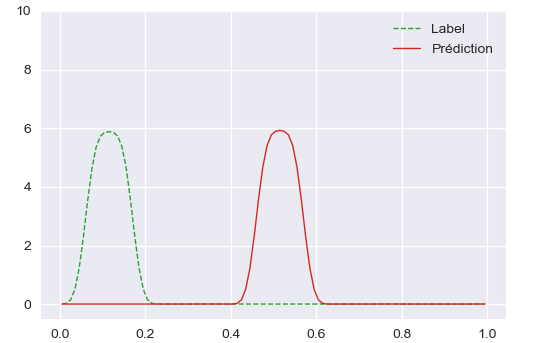
\includegraphics[width=4cm]{Pire1D1}       
        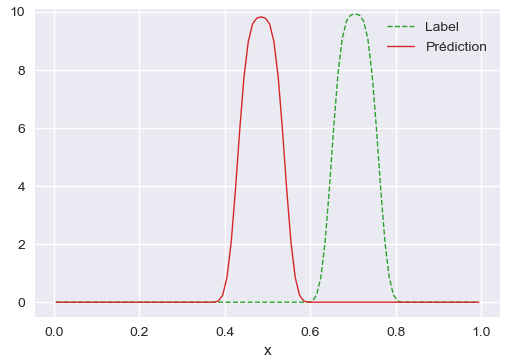
\includegraphics[width=4cm]{Pire1D2}       
        \caption{Les pires predictions}
        \end{figure}
     \end{column}
    \end{columns}

\end{frame}

\begin{frame}
    \frametitle{Scores 1D}

    \begin{table}[h!]
        \caption{Scores 1D}
        \centering
        \begin{tabular}{l l}
        \toprule
        \textbf{Nom du score} & \textbf{Valeur} \\
        \midrule
        R2 & 99.50 \%\\
        Personnalisé & 28.21 \%\\
        \bottomrule\\
        \end{tabular}
    \end{table}

    \begin{columns}
        \begin{column}{0.5\textwidth}
            \begin{figure}
            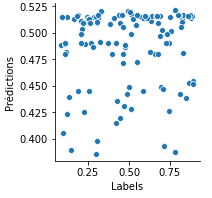
\includegraphics[width=2cm]{Position1D}       
            \caption{Correlation des position}
            \end{figure}
         \end{column}
         \begin{column}{0.5\textwidth}
            \begin{figure}
            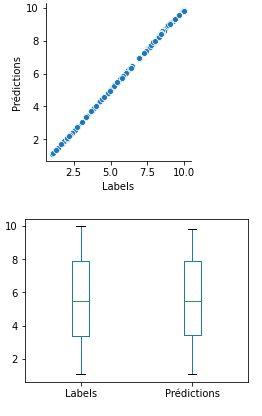
\includegraphics[width=2cm]{Hauteur1D}       
            \caption{Correlation des hauteur}
            \end{figure}
         \end{column}
    \end{columns}

\end{frame}


\begin{frame}
    \frametitle{Conclusion sur la régression 1D}
Les cause de l'echec:
\begin{itemize}
    \item Le probleme inverse est probablement mal pose  % EN supposant que je n'ai commise aucune erreur
    \item Le score R2 est mal calcule % Non prise en compte des poinds 10:1. 
\end{itemize}
\end{frame}


% \end{document}
